\begin{flushright} {\tiny {\color{gray} mms\_channelHB.tex}} \end{flushright}
%~~~~~~~~~~~~~~~~~~~~~~~~~~~~~~~~~~~~~~~~~~~~~~~~~~~~~~~~~~~~~~~~~~~~~~~~~~~~~~~~~~~~~~~~~~~~~~~~~~


We start from the following formulation for the Herschel-Bulkley rheology:
\begin{mdframed}[backgroundcolor=blue!5]
\[
\eta_{HB}
=
\left\{
\begin{array}{lc}
\eta_0 & \dot{\varepsilon}_e\leq \dot{\varepsilon}_0 \\
K  \dot{\varepsilon}_e^{n-1} + \frac{\tau_0}{\dot{\varepsilon}_e}  
& \dot{\varepsilon}_e\geq \dot{\varepsilon}_0 
\end{array}
\right.
\]
\end{mdframed}
and the limiting viscosity $\eta_0$ is such that 
\[
\eta_0 = K  \dot{\varepsilon}_0^{n-1} + \frac{\tau_0}{\dot{\varepsilon}_0}  
\]

We consider a two-dimensional channel in the $x,y$ plane. The walls 
are at $y=0$ and $y=H$ with no-slip boundary conditions. 
In the absence of gravity, the Stokes equation simplify to 
\begin{equation}
-\frac{\partial p}{\partial x}  +\frac{\partial }{\partial y} (2\eta_{HB} \dot{\varepsilon}_{xy}) =0
\qquad
\text{and}
\qquad
\dot{\varepsilon}_{xy} = \frac{1}{2} \frac{\partial u}{\partial y} 
\label{eq:hb1}
\end{equation}
where we assume the velocity $\vec\upnu=(u(y),0)$.
It then follows that 
\[
\dot{\varepsilon}_{e} 
= \sqrt{{\III}_2(\dot{\bm \varepsilon})} 
=\sqrt{ \frac{1}{2} \dot{\bm \varepsilon} : \dot{\bm \varepsilon} }
=\sqrt{ 
\frac{1}{2}[(\dot{\varepsilon}_{xx})^2 + (\dot{\varepsilon}_{yy})^2 + (\dot{\varepsilon}_{zz})^2]  
+ (\dot{\varepsilon}_{xy})^2  
+ (\dot{\varepsilon}_{xz})^2  
+ (\dot{\varepsilon}_{yz})^2 
}
=\sqrt{\dot{\varepsilon}_{xy}^2 }
= \left|\frac{1}{2} \frac{\partial u}{\partial y}  \right|
\]
In the case of a Newtonian fluid, the analytical solution is 
known and the velocity profile is a parabola with zero velocity on the
walls and maximum velocity in the middle. 
Although the rheology of the fluid is non-linear we assume that a 
similar velocity profile is expected (although not described by a parabola).
We then expect three zones (and we assume that the fluid flows from left to right):
\begin{itemize}

%..............................
\item In the middle, where it is expected that $\frac{\partial u}{\partial y}=0$ (at least in one point)
because of symmetry. We also therefore expect $\dot{\varepsilon}_e\leq \dot{\varepsilon}_0$ in this region
so that $\eta_{HB}=\eta_0$. How thick this region is will be determined later. 

Eq.~\eqref{eq:hb1} must then be solved 
\begin{eqnarray}
\frac{\partial p}{\partial x}  
&=&\frac{\partial }{\partial y} \left(2\eta_{HB}  \frac{1}{2}\frac{\partial u}{\partial y} \right) 
= \eta_0 \frac{\partial^2 u}{\partial y^2}  
\end{eqnarray}

Let us call $\Pi=\frac{\partial p}{\partial x} <0$, then we must solve:
\[
\frac{\partial^2 u}{\partial y^2} = \frac{\Pi}{\eta_0} 
\]
The solution is then of the form
\[
\boxed{
u(y)|_{mid} = \frac{1}{2}\frac{\Pi}{\eta_0} y^2 + 2a y + b
}
\]
and 
\[
\boxed{
\dot{\varepsilon}_{xy}|_{mid}= \frac{1}{2} \frac{\Pi}{\eta_0}y  + a
}
\]
We will determine $a$ and $b$ later. 

%..............................
\item Near the bottom wall, with $\frac{\partial u}{\partial y}>0$ so that  
$\dot{\varepsilon}_{e} = +\frac{1}{2}\left( \frac{\partial u}{\partial y}  \right)$  
and $\dot{\varepsilon}_e\geq \dot{\varepsilon}_0 $. 
We solve Eq.~\eqref{eq:hb1} again, this time with the non-linear formulation of the viscosity: 
\begin{eqnarray}
\frac{\partial p}{\partial x}  
&=&\frac{\partial }{\partial y} \left( 2 \eta_{HB}  \frac{1}{2}\frac{\partial u}{\partial y} \right)  \nn\\
&=&2 \frac{\partial }{\partial y} \left[  
\left( K  \dot{\varepsilon}_e^{n-1} + \frac{\tau_0}{\dot{\varepsilon}_e}  
\right) \frac{1}{2}\frac{\partial u}{\partial y} \right] \nn\\
&=&2\frac{\partial }{\partial y} \left[  
\left( K \left|\frac{1}{2}\frac{\partial u}{\partial y}\right|^{n-1} 
+ \tau_0 \left|\frac{1}{2}\frac{\partial u}{\partial y}\right|^{-1} 
\right) \frac{1}{2}\frac{\partial u}{\partial y} \right]  \nn\\
&=& 2 \frac{\partial }{\partial y} \left[  
K \left(\frac{1}{2}\frac{\partial u}{\partial y}\right)^{n} + \tau_0 \right] 
\end{eqnarray}
We then must solve:
\[
\frac{\partial }{\partial y} \left[  
K \left(\frac{1}{2}\frac{\partial u}{\partial y}\right)^{n} + \tau_0 \right] 
= \frac{\Pi}{2}
\]
\[
K \left(\frac{1}{2}\frac{\partial u}{\partial y}\right)^{n} + \tau_0  = \frac{\Pi}{2} y +c
\]
\[
\left(\frac{1}{2}\frac{\partial u}{\partial y}\right)^{n}   = \frac{1}{K} ( \frac{\Pi}{2} y +c -\tau_0 )
\]
or, 
\[
\boxed{
\dot{\varepsilon}_{xy}|_{bot}=
\frac{1}{2}\frac{\partial u}{\partial y}  = \left( \frac{1}{K} ( \Pi_2 y +c -\tau_0 ) \right)^{1/n}
}
\]
so 
\[
\boxed{
u(y)|_{bot} = 2 \frac{n}{n+1} \frac{K}{\Pi_2} \left( \frac{1}{K} ( \Pi_2 y +c -\tau_0 ) \right)^{1+1/n} + d
}
\]
where $\Pi_2=\Pi/2$

%..............................
\item Near the top wall, with $\frac{\partial u}{\partial y}<0$ so that 
$\dot{\varepsilon}_{e} = -\frac{1}{2}\left( \frac{\partial u}{\partial y}  \right)$ 
and $\dot{\varepsilon}_e\geq \dot{\varepsilon}_0$. We solve yet again Eq.~\eqref{eq:hb1}:
\begin{eqnarray}
\frac{\partial p}{\partial x}  
&=&\frac{\partial }{\partial y} \left( 2 \eta_{HB}  \frac{1}{2}\frac{\partial u}{\partial y} \right)  \nn\\
&=&2 \frac{\partial }{\partial y} \left[  
\left( K  \dot{\varepsilon}_e^{n-1} + \frac{\tau_0}{\dot{\varepsilon}_e}  
\right) \frac{1}{2}\frac{\partial u}{\partial y} \right] \nn\\
&=&2\frac{\partial }{\partial y} \left[  
\left( K \left|\frac{1}{2}\frac{\partial u}{\partial y}\right|^{n-1} 
+ \tau_0 \left|\frac{1}{2}\frac{\partial u}{\partial y}\right|^{-1} 
\right) \frac{1}{2}\frac{\partial u}{\partial y} \right]  \nn\\
&=&-2\frac{\partial }{\partial y} \left[  
\left( K \left( - \frac{1}{2}\frac{\partial u}{\partial y}\right)^{n-1} 
+ \tau_0 \left( -\frac{1}{2}\frac{\partial u}{\partial y}\right)^{-1} 
\right) \left(-\frac{1}{2}\frac{\partial u}{\partial y}\right) \right]  \nn\\
&=& -2\frac{\partial }{\partial y} \left[   
K \left(-\frac{1}{2}\frac{\partial u}{\partial y}\right)^{n} + \tau_0 \right] 
\end{eqnarray}
We then must solve:
\[
-\frac{\partial }{\partial y} \left[ 
K \left(-\frac{1}{2}\frac{\partial u}{\partial y}\right)^{n} + \tau_0 \right] 
= \frac{\Pi}{2}
\]
\[
K \left(-\frac{1}{2}\frac{\partial u}{\partial y}\right)^{n} + \tau_0 = - \frac{\Pi}{2} y + e
\]
\[
 \left(-\frac{1}{2}\frac{\partial u}{\partial y}\right)^{n}  = \frac{1}{K} (-\frac{\Pi}{2} y + e - \tau_0)
\]
which yields
\[
\boxed{
\dot{\varepsilon}_{xy}|_{top}
=  - \left( \frac{1}{K} (- \Pi_2 y +e - \tau_0 ) \right)^{1/n}
}
\]
\[
\boxed{
u(y)|_{top} = 2 \frac{n}{n+1} \frac{K}{\Pi_2} \left( \frac{1}{K} ( -\Pi_2 y +e -\tau_0 ) \right)^{1+1/n} + f
}
\]


\end{itemize}

\newpage

We have 6 integration constants $a,b,c,d,e,f$ and 6 additional constraints from 
continuity or boundary conditions:
\begin{eqnarray}
(1)&&u(0) = 0 \text{ boundary condition}\\
(2)&&u(H) = 0 \text{ boundary condition}\\
(3)&&u(y_1) \text{ must be continuous}\\
(4)&&u(y_2) \text{ must be continuous}\\
(5)&&\dot{\varepsilon}_{xy}(y_1) \text{ must be continuous}\\
(6)&&\dot{\varepsilon}_{xy}(y_2) \text{ must be continuous}
\end{eqnarray}

%......................................................
\paragraph{Using symmetry to compute $a$}
Because of symmetry, we expect $y_1=H/2-\delta$ and $y_2=H/2+\delta$ with $\delta \neq 0$ 
(i.e. $y_1\neq y_2$) and we expect $u(y_1)=u(y_2)$ so that 
\[
u(y_1)|_{mid}=
\frac{1}{2}\frac{\Pi}{\eta_0} y_1^2 + 2a y_1 + b
=
\frac{1}{2}\frac{\Pi}{\eta_0} y_2^2 + 2a y_2 + b=
u(y_2)|_{mid}
\]
or, 
\[
\frac{1}{2}\frac{\Pi}{\eta_0} (y_1^2-y_2^2) + 2a (y_1-y_2) =0
\]
\[
\frac{1}{2}\frac{\Pi}{\eta_0} (y_1-y_2)(y_1+y_2) + 2a (y_1-y_2) =0
\]
\[
\frac{1}{2}\frac{\Pi}{\eta_0} (y_1+y_2) + 2a =0
\]
\[
\frac{1}{2}\frac{\Pi}{\eta_0} H + 2a =0
\]
and finally we obtain $a$:
\[
\boxed{
a = -\frac{1}{4} \frac{\Pi}{\eta_0} H
}
\]
Note that we could have obtained the same thing by enforcing that the strain rate 
at $y_1$ and $y_2$ are the opposite of one another. It then follows: 
\[
\boxed{
u(y)|_{mid} 
= \frac{1}{2}\frac{\Pi}{\eta_0} y^2  -2\frac{1}{4} \frac{\Pi}{\eta_0} H y + b
= \frac{1}{2}\frac{\Pi}{\eta_0} (y^2  -  y H) + b
= \frac{\Pi_2}{\eta_0} (y^2  -  y H) + b
}
\]
and 
\[
\boxed{
\dot{\varepsilon}_{xy}|_{mid}
= \frac{1}{2} \frac{\Pi}{\eta_0}y  -\frac{1}{4} \frac{\Pi}{\eta_0} H
= \frac{1}{2} \frac{\Pi}{\eta_0} (y  -\frac{H}{2} )
=  \frac{\Pi_2}{\eta_0} (y  -\frac{H}{2} )
}
\]
Because of the parabola-like flow profile, we expect the strain rate 
to be zero in the middle $y=H/2$, and positive for $z_1<y<H/2$ and 
negative for $H/2<y<z_2$, which is indeed what we recover ($\Pi<0$).

%......................................................
\paragraph{Using bottom boundary condition to obtain $d$}
\[
u(y=0)|_{bot} = 2 \frac{n}{n+1} \frac{K}{\Pi_2} \left( \frac{1}{K} ( c -\tau_0 ) \right)^{1+1/n} + d = 0
\]
so 
\[
d = -2 \frac{n}{n+1} \frac{K}{\Pi_2} \left( \frac{1}{K} ( c -\tau_0 ) \right)^{1+1/n} 
\]
and then
\[
\boxed{
u(y)|_{bot} = 
2 \frac{n}{n+1} \frac{K}{\Pi_2} \left[ \left( \frac{1}{K} ( \Pi y +c -\tau_0 ) \right)^{1+1/n} 
- \left( \frac{1}{K} ( c -\tau_0 ) \right)^{1+1/n} \right]
}
\]


%......................................................
\paragraph{Using top boundary condition to obtain $f$}
\[
u(y=H)|_{top} = 2 \frac{n}{n+1} \frac{K}{\Pi_2} \left( \frac{1}{K} ( -\Pi_2 H +e -\tau_0 ) \right)^{1+1/n} + f =0
\]
so 
\[
f= -2 \frac{n}{n+1} \frac{K}{\Pi_2} \left( \frac{1}{K} ( -\Pi_2 H +e -\tau_0 ) \right)^{1+1/n} 
\]
and then
\[
\boxed{
u(y)|_{top} = 2 \frac{n}{n+1} \frac{K}{\Pi_2}
\left[
\left( \frac{1}{K} ( -\Pi_2 y +e -\tau_0 ) \right)^{1+1/n} - 
\left( \frac{1}{K} ( -\Pi_2 H +e -\tau_0 ) \right)^{1+1/n} \right]
}
\]


%......................................................
\paragraph{computing $\delta$}

The coordinates of the transitions $y_1$ and $y_2$ are the location where the strain rate
$\dot{\varepsilon}_e$ reaches $\dot{\varepsilon}_0$. In other words:
\[
\dot{\varepsilon}_{e}|_{mid}(y=y_1) = 
\dot{\varepsilon}_{xy}|_{mid}(y=y_1)  
= \frac{1}{2} \frac{\Pi}{\eta_0} \left(y_1  -\frac{H}{2} \right)
= \frac{1}{2} \frac{\Pi}{\eta_0} \left(\frac{H}{2}-\delta  -\frac{H}{2} \right)
= -\frac{1}{2} \frac{\Pi}{\eta_0} \delta
= \dot{\varepsilon}_0
\]
or, 
\[
\delta = -\frac{2 \dot{\varepsilon}_0 \eta_0}{\Pi}
\]
Since $\Pi<0$ it adds up and $\delta>0$. We can also write
\[
\boxed{
\delta = \frac{2 \dot{\varepsilon}_0 \eta_0}{|\Pi|}
}
\]
and we will use throughout what follows:
\[
\dot{\varepsilon}_0 = - \frac{1}{2}\frac{\Pi}{\eta_0} \delta
\]


%......................................................
\paragraph{Using strain rate continuity at $y_1$ to compute $c$}
\[
\left( \frac{1}{K} ( \Pi_2 y_1 +c -\tau_0 ) \right)^{1/n}
= \frac{1}{2} \frac{\Pi}{\eta_0} \left(y_1  -\frac{H}{2} \right)
=- \frac{1}{2} \frac{\Pi}{\eta_0} \delta
\]
\[
 \Pi_2 y_1 +c -\tau_0 
= K\left( - \frac{1}{2} \frac{\Pi}{\eta_0} \delta\right)^{n}
\]
\[
c = K\left( - \frac{1}{2} \frac{\Pi}{\eta_0} \delta\right)^{n} + \tau_0 -\Pi_2 y_1
\]

\[
\boxed{
c = K \dot{\varepsilon}_0^{n} + \tau_0 -\Pi_2 y_1
}
\]




\begin{eqnarray}
u(y)|_{bot} 
&=& 
2 \frac{n}{n+1} \frac{K}{\Pi_2} \left[ \left( \frac{1}{K} ( \Pi_2 y +c -\tau_0 ) \right)^{1/n+ 1 } 
- \left( \frac{1}{K} ( c -\tau_0 ) \right)^{1/n+ 1 } \right]
\nn\\
&=& 2 \frac{n}{n+1} \frac{K}{\Pi_2} 
\left[ \left( \frac{1}{K} ( \Pi_2 (y-y_1) +K \dot{\varepsilon}_0^{n}   ) \right)^{1/n+ 1 } 
- \left( \frac{1}{K} (  K  
\dot{\varepsilon}_0^{n}  -\Pi_2 y_1    ) \right)^{1/n+ 1 } \right]
\nn\\
&=& 
2 \frac{n}{n+1} \frac{K}{\Pi_2} \left[ \left( \frac{\Pi_2}{K} (y-y_1) 
+ \dot{\varepsilon}_0^{n}    \right)^{1/n+ 1 } 
- \left(  \dot{\varepsilon}_0^{n}  - \frac{\Pi_2}{K}y_1     \right)^{1/n+ 1 } \right]
\nn\\
\dot{\varepsilon}_{xy}|_{bot}
&=& \left( \frac{1}{K} ( \Pi_2 y +c -\tau_0 ) \right)^{1/n} \nn\\
&=& \left( \frac{\Pi_2}{K} (y-y_1) + \dot{\varepsilon}_0^{n}   \right)^{1/n} \nn
\end{eqnarray}



%......................................................
\paragraph{Using strain rate continuity at $y_2$ to compute $e$}
\[
-\left( \frac{1}{K} ( -\Pi_2 y_2 +e -\tau_0 ) \right)^{1/n}
= \frac{1}{2} \frac{\Pi}{\eta_0} \left(y_2  -\frac{H}{2} \right)
= \frac{1}{2} \frac{\Pi}{\eta_0} \delta  
\]
\[
-\Pi_2 y_2 +e -\tau_0 
= K\left(-\frac{1}{2} \frac{\Pi}{\eta_0} \delta  \right)^{n} 
\]
\[
e = K\left(-\frac{1}{2} \frac{\Pi}{\eta_0} \delta  \right)^{n} + \tau_0 + \Pi_2 y_2 
\]
\[
\boxed{
e = K \dot{\varepsilon}_0^n + \tau_0 + \Pi_2 y_2 
}
\]

\begin{eqnarray}
u(y)|_{top} &=& 2 \frac{n}{n+1} \frac{K}{\Pi_2}
\left[
\left( \frac{1}{K} ( -\Pi_2 y +e -\tau_0 ) \right)^{1/n+ 1 } - 
\left( \frac{1}{K} ( -\Pi_2 H +e -\tau_0 ) \right)^{1/n+ 1 } \right] \nn\\
&=& 2 \frac{n}{n+1} \frac{K}{\Pi_2}
\left[
\left( -\frac{\Pi_2}{K}(y-y_2)+ \dot{\varepsilon}_0^{n}  \right)^{1/n+ 1 } - 
\left( -\frac{\Pi_2}{K}(H-y_2)+ \dot{\varepsilon}_0^{n}  \right)^{1/n+ 1 } 
\right]
\nn\\
\dot{\varepsilon}_{xy}|_{top}
&=&  - \left( \frac{1}{K} (- \Pi_2 y +e - \tau_0 ) \right)^{1/n} \nn\\
&=&  - \left( - \frac{\Pi_2}{K} (y-y_2) +  \dot{\varepsilon}_0^{n} \right)^{1/n} \nn
\end{eqnarray}

%......................................................
\paragraph{Using velocity continuity to compute $b$} 
We use $u(y_1)|_{bot}=u(y_1)|_{mid}$: 

\[
2 \frac{n}{n+1} \frac{K}{\Pi_2} \left[ \left( \frac{\Pi_2}{K} (y_1-y_1) 
+ \dot{\varepsilon}_0^{n}    \right)^{1/n+ 1 } 
- \left( \dot{\varepsilon}_0^{n}  - \frac{\Pi_2}{K}y_1     \right)^{1/n+ 1 } \right]
=
\frac{\Pi_2}{\eta_0} (y_1^2  -  y_1 H) + b
\]

\[
2 \frac{n}{n+1} \frac{K}{\Pi_2} \left[ 
\dot{\varepsilon}_0^{n+ 1} 
- \left( \dot{\varepsilon}_0^{n}  - \frac{\Pi_2}{K}y_1  \right)^{1/n+ 1 } \right]
=
\frac{\Pi_2}{\eta_0} y_1 (y_1  - H) + b
\]
so 
\[
b= 
2 \frac{n}{n+1} \frac{K}{\Pi_2} \left[ 
\dot{\varepsilon}_0^{n+ 1} 
- \left( \dot{\varepsilon}_0^{n}  - \frac{\Pi_2}{K}y_1  \right)^{1/n+ 1 } \right]
- \frac{\Pi_2}{\eta_0} y_1 (y_1  - H) 
\]

%..............................................................
\paragraph{Using velocity continuity to compute $b$ (again?)} 
This time we use $u(y_2)|_{top}=u(y_2)|_{mid}$: 

\[
2 \frac{n}{n+1} \frac{K}{\Pi_2}
\left[
\left( -\frac{\Pi_2}{K}(y_2-y_2)+ \dot{\varepsilon}_0^{n}  \right)^{1/n+ 1 } - 
\left( -\frac{\Pi_2}{K}(H-y_2)+ \dot{\varepsilon}_0^{n}  \right)^{1/n+ 1 } 
\right]
= \frac{\Pi_2}{\eta_0} (y_2^2  -  y_2 H) + b
\]

\[
2 \frac{n}{n+1} \frac{K}{\Pi_2}
\left[
\dot{\varepsilon}_0^{n+1}  - 
\left( -\frac{\Pi_2}{K}(H-y_2)+   \dot{\varepsilon}_0^{n}  \right)^{1/n+ 1 } 
\right]
=
\frac{\Pi_2}{\eta_0} (y_2^2  -  y_2 H) + b
\]
and since $H-y_2 = H- H/2 - \delta = H/2 -\delta = y_1$ and
\[
y_2^2-y_2H = y_2(y_2 - H) = (H/2+\delta)(-y_1) 
= (-H/2-\delta)y_1
= (-H+H/2-\delta)y_1
= (-H+y_1)y_1
\] 
so that we indeed recover the same $b$ value as above. 

\newpage
To summarize:

\begin{mdframed}[backgroundcolor=blue!5]
\begin{eqnarray}
u(y)|_{bot} 
&=& 
2 \frac{n}{n+1} \frac{K}{\Pi_2} \left[ \left( \frac{\Pi_2}{K} (y-y_1) +  \dot{\varepsilon}_0^{n}    \right)^{1/n+ 1 } 
- \left(   \dot{\varepsilon}_0^{n}  - \frac{\Pi_2}{K}y_1     \right)^{1/n+ 1 } \right]
\nn\\
u(y)|_{mid} 
&=& \frac{\Pi_2}{\eta_0} (y^2  -  y) + 
2 \frac{n}{n+1} \frac{K}{\Pi_2} \left[ 
+ \dot{\varepsilon}_0^{n+ 1} 
- \left( \dot{\varepsilon}_0^{n}  - \frac{\Pi_2}{K}y_1  \right)^{1/n+ 1 } \right]
- \frac{\Pi_2}{\eta_0} y_1 (y_1  - H) 
\nn\\
u(y)|_{top} 
&=& 2 \frac{n}{n+1} \frac{K}{\Pi_2}
\left[
\left(-\frac{\Pi_2}{K}(y+y_2)+ \dot{\varepsilon}_0^{n}\right)^{\frac{1}{n}+ 1 } - 
\left(-\frac{\Pi_2}{K}(H+y_2)+ \dot{\varepsilon}_0^{n}\right)^{\frac{1}{n}+ 1 } 
\right]
\nn\\
\dot{\varepsilon}_{xy}|_{bot}
&=& \left( \frac{\Pi_2}{K} (y-y_1) + \dot{\varepsilon}_0^{n}   \right)^{1/n} \nn\\
\dot{\varepsilon}_{xy}|_{mid}
&=& \frac{\Pi_2}{\eta_0} (y  -\frac{H}{2} ) \nn\\
\dot{\varepsilon}_{xy}|_{top}
&=&  - \left( - \frac{\Pi_2}{K} (y-y_2) +  \dot{\varepsilon}_0^{n} \right)^{1/n} \nn
\end{eqnarray}
\end{mdframed}

Rather interestingly we find that $\tau_0$ does not directly enter the equations above.
This can be explained as follows: since we have the relationship 
\[
\eta_0 = K \dot{\varepsilon}_0^{n-1}  + \frac{\tau_0}{\dot{\varepsilon}_0}  
\]
the parameters $\eta_0$, $\dot{\varepsilon}_0$, $\tau_0$ and $K$ cannot be all chosen freely.
The viscosity $\eta_0$ is reached when the strain rate becomes smaller than $\dot{\varepsilon}_0$, 
so these two parameters have a physical meaning. We set $\eta_0=10^{25}$ and 
$\dot{\varepsilon}_0=10^{-17}$. When/if $K$ is zero, then $\tau_0$ can be interpreted as a 
yield value for a rigid plastic material so we arbitrarily set it to $\tau_0 = 10^7$. 
Having fixed these parameters we can compute 
\[
K= \frac{\eta_0 \dot{\varepsilon}_0 - \tau_0}{ \dot{\varepsilon}_0^n}
\] 

The data used to produce all the following plots is generated by the python program and a gnuplot script 
to be found in {\tt images/mms/channel\_hb/}.

%............................................................
\paragraph{Let's start simple: $n=1$}

In this case the viscosity is given by 
\[
\eta_{HB}
=
\left\{
\begin{array}{lc}
\eta_0 & \dot{\varepsilon}_e\leq \dot{\varepsilon}_0 \\
K+ \frac{\tau_0}{\dot{\varepsilon}_e}   & \dot{\varepsilon}_e\geq \dot{\varepsilon}_0 
\end{array}
\right.
\]
%and the limiting viscosity $\eta_0$ is such that 
%\[
%\eta_0 = K  + \frac{\tau_0}{\dot{\varepsilon}_0}  
%\]
Since $\dot{\varepsilon}_e = \left|\frac{1}{2}\frac{\partial u}{\partial y} \right|$
then 
\[
\eta_{HB}
=
\left\{
\begin{array}{lc}
\eta_0 & \dot{\varepsilon}_e\leq \dot{\varepsilon}_0 \\
K+ \frac{2\tau_0}{  \left| \frac{\partial u}{\partial y} \right|  }   & \dot{\varepsilon}_e\geq \dot{\varepsilon}_0 
\end{array}
\right.
\]

\begin{center}
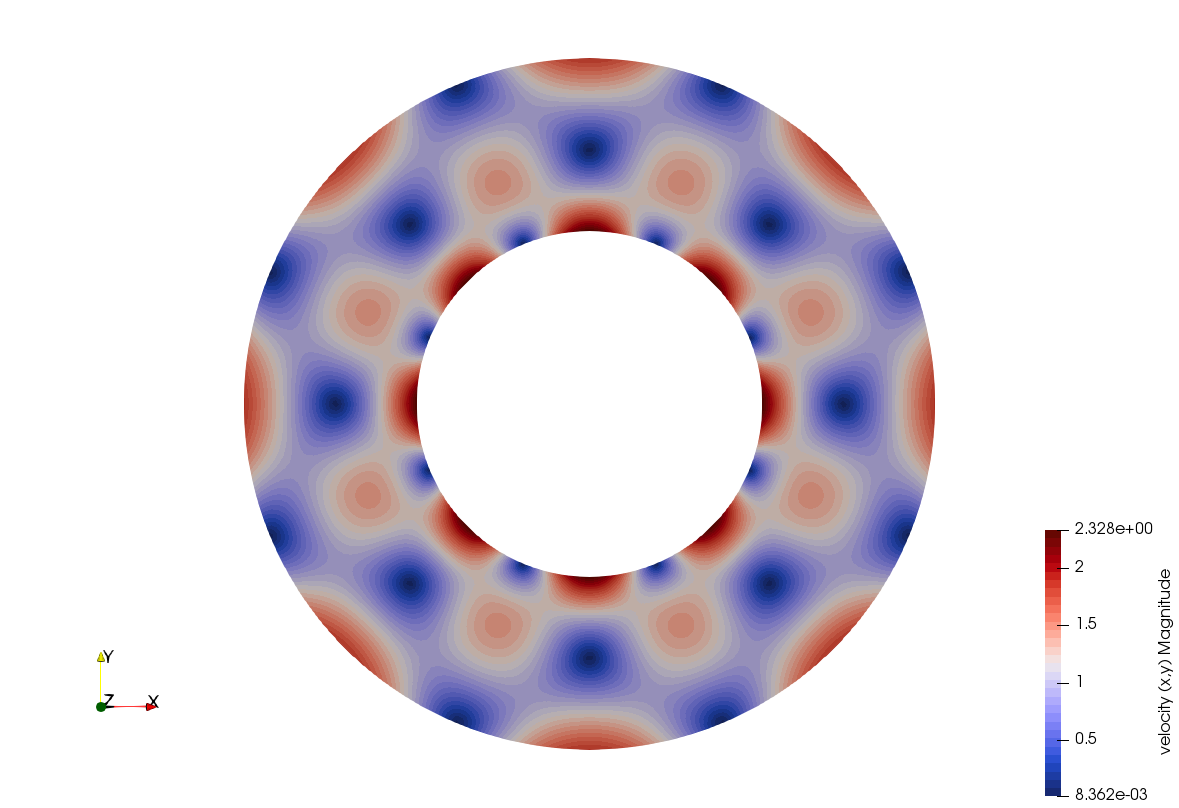
\includegraphics[width=7cm]{images/mms/channel_hb/velocity}
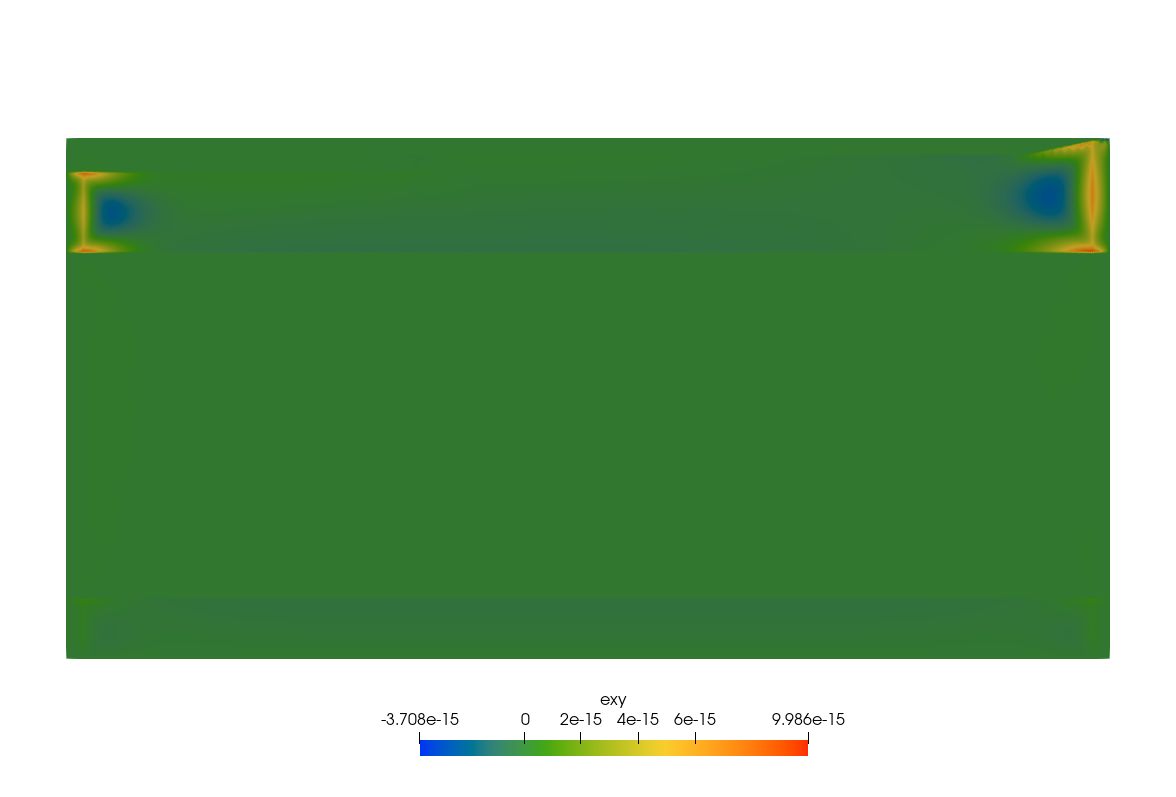
\includegraphics[width=7cm]{images/mms/channel_hb/exy}\\
{\captionfont Obtained for $n=1$ and $\tau_0=9e7$. The black lines are the resulting velocity and strain rate profiles obtained by joining the bottom, middle and top functions.}
\end{center}

In the following I explore the effect of the $\tau_0$ value ($K$ is calculated correspondingly as we have seen before).

\begin{center}
\includegraphics[width=7.5cm]{images/mms/channel_hb/velocity_taus}
\includegraphics[width=7.5cm]{images/mms/channel_hb/exy_taus}\\
\includegraphics[width=7.5cm]{images/mms/channel_hb/ee_taus}
\includegraphics[width=7.5cm]{images/mms/channel_hb/eta_taus}
\end{center}




